% !TeX root = er.tex

\chapter{Localization}\label{ch.local}

A navegação por odometria (Sect.~\ref{s.odometry}) é propensa a erros e só pode dar uma estimativa da real pose do robô. Além disso, quanto mais o robô se move, maior é o erro na estimativa da pose, especialmente no cabeçalho. A odometria em um robô pode ser comparada a caminhar de olhos fechados, contando passos até chegarmos ao nosso destino. Como na odometria, quanto mais avançamos, mais incertos estamos quanto à nossa localização. Mesmo ao contar passos, devemos abrir nossos olhos de vez em quando para reduzir a incerteza de nossa localização. Para um robô, o que significa "contar passos" e "abrir nossos olhos de tempos em tempos"? Significa que para mover distâncias curtas a odometria é suficientemente boa, mas ao mover distâncias maiores o robô deve determinar sua posição em relação a uma referência externa chamada marco. Este processo é chamado de \emph{localização}.

A seção {s.marcos} começa com uma atividade que você pode usar para se familiarizar com a relação entre odometria e localização. A seção~\ref{s.known-points} apresenta técnicas trigonométricas clássicas usadas por topógrafos para determinar a posição de um local na terra, medindo ângulos e distâncias a posições cuja localização é conhecida. A seção~\ref{s.gps} pesquisa brevemente os sistemas de posicionamento global (GPS) que agora são amplamente utilizados para localização. Há ambientes onde o GPS não é eficaz: em edifícios e quando são necessárias posições muito precisas. Os robôs nestes ambientes utilizam técnicas de localização probabilística que são descritas em Sects.~\ref{s.prob-local}--\ref{s.uncertain-motion}.

\section{Pontos de referência}\label{s.landmarks}

Pontos de referência, como linhas no chão ou portas em um corredor, podem ser detectados e identificados pelo robô e utilizados para localização. A seguinte atividade - que não usa nem computador nem robô - ajudará a entender a importância de identificar pontos de referência para corrigir erros de odometria.

\begin{framed}
\act{Jogue o jogo do marco}{landmark-game}
\begin{itemize}
\item Escolha um caminho em sua casa que exija que você passe várias portas, por exemplo, da cama em seu quarto através de um corredor até um sofá na sala de estar e depois volte.
\item Feche os olhos e caminhe ao longo do caminho aplicando as seguintes regras
\begin{itemize}
\item Você recebe $30$ pontos no início da atividade.
\item De tempos em tempos você pode abrir os olhos por um segundo; esta ação custa $1$ ponto.
\item Se você tocar uma parede, isso custa $10$ pontos.
\end{itemize}
\item Quantos pontos você tem quando completa o caminho?
\item É melhor abrir os olhos com freqüência ou percorrer o caminho sem nunca abrir os olhos?
\end{itemize}
\end{framed}

\section[posição a partir de objetos cuja posição é conhecida]{Determinação da posição a partir de objetos cuja posição é conhecida}\label{s.known-points}

Nesta seção descrevemos dois métodos que um robô pode utilizar para determinar sua posição medindo ângulos e distâncias a um objeto cuja posição é conhecida. O primeiro método assume que o robô pode medir a distância até o objeto e seu \emph{azimute}, o ângulo do objeto em relação ao norte. O segundo método mede os ângulos para o objeto a partir de duas posições diferentes. Ambos os métodos utilizam a trigonometria para calcular as coordenadas do robô em relação ao objeto. Se as coordenadas absolutas $(x_0,y_0)$ do objeto forem conhecidas, as coordenadas absolutas do robô podem então ser facilmente computadas.

\subsection{Determinação da posição a partir de um ângulo e de uma distância}

A figura~\ref{fig.angle-distance} mostra a geometria de um robô em relação a um objeto. No diagrama, o objeto é indicado pelo ponto grande colocado na origem $(x_0,y_0)$ de um sistema de coordenadas. O azimute do robô $\theta$ é o ângulo entre o norte e a direção de avanço do robô; ele pode ser medido por uma bússola. Um scanner laser é usado para medir a distância $s$ ao objeto e o ângulo $\phi$ entre a direção para frente do robô e o objeto. As coordenadas relativas $\Delta x$ e $\Delta y$ podem ser determinadas por trigonometria simples:
\[
\Delta x = s \sin (\theta-\phi), \;\;\; \Delta y = s \cos (\theta-\phi)\,.
\]
A partir das coordenadas absolutas conhecidas do objeto $(x_0,y_0)$, as coordenadas do robô podem ser determinadas.

\begin{figure}
\begin{center}
\begin{tikzpicture}[scale=1.2]
\draw (-1,3) -- node[above] { $\Delta x$ } +(7,0);
\pic[rotate=15,scale=.8] at (0,0) { robot };
\draw[dashed] (0,0) -- +(15:6cm);
\draw[dashed] (0,0) -- +(30:7cm);
\draw (0,0) -- node[left] { $\Delta y$ } +(90:4cm);
\draw (5.2,0) -- +(0,4);
\draw[fill] (5.2,3) circle [radius=2pt];
\draw[red,thick] (0,2.3cm) arc[radius=2.3cm, start angle=90, delta angle = -75];
\draw[blue,thick] (30:3.1cm)  arc[radius=3.1cm, start angle=30, delta angle = -15];
\draw[thick] (90:1.5cm) arc[radius=1.5cm, start angle=90, delta angle = -60];
\node at (5.7,2.8) { $(x_0,y_0)$ };
\node at (60:2.6cm) { $\theta$ };
\node at (60:1.8cm) { $\theta-\phi$ };
\node at (22.5:3.3) { $\phi$ };
\end{tikzpicture}
\caption{Determinação da posição a partir de um ângulo e de uma distância}\label{fig.angle-distance}
\end{center}
\end{figure}

\begin{framed}
\act{Determinação da posição a partir de um ângulo e de uma distância}{position-distance-angle}
\begin{itemize}
\item Implementar o algoritmo.
\item Para medir o azimute, coloque o robô alinhado com uma borda da mesa e chame-o de norte. Meça o ângulo até o objeto usando vários sensores horizontais ou usando um sensor e girando ou o sensor ou o robô.
\item A distância e o ângulo são medidos a partir da posição onde o sensor é montado, que não é necessariamente o centro do robô. Talvez você tenha que fazer correções para isso.
\end{itemize}
\end{framed}

\subsection{Determinação da posição por triangulação}

\emph{Triangulação} é usada para determinar coordenadas quando é difícil ou impossível medir distâncias. Era amplamente utilizada em levantamentos antes que os lasers estivessem disponíveis, pois era impossível medir distâncias longas com precisão. O princípio da triangulação é que a partir de dois ângulos de um triângulo e do comprimento do lado incluído, é possível calcular os comprimentos dos outros lados. Uma vez que estes são conhecidos, a posição relativa de um objeto distante pode ser computada.

A figura~\ref{fig.triangulation} mostra o robô medindo os ângulos $\alpha$ e $\beta$ ao objeto a partir de duas posições separadas por uma distância $c$. Se as duas posições estiverem próximas, a distância pode ser medida usando uma fita métrica. Alternativamente, a distância pode ser medida por odometria à medida que o robô se move de uma posição para outra, embora isto possa ser menos preciso. Na topografia, se as coordenadas das duas posições forem conhecidas, a distância entre elas pode ser calculada e usada para determinar as coordenadas do objeto.

Os comprimentos $a$ e $b$ são computados usando a \emph{law of sines}:
\begin{displaymath}
\frac{a}{\sin\alpha'} = \frac{b}{\sin\beta'} = \frac{c}{\sin\gamma}\,,
\end{displaymath}
onde $\alpha' = 90^\circ{} - \alpha, \beta' = 90^\circ{} \beta$ são os ângulos interiores do triângulo. Para usar a lei, precisamos $c$, que foi medido, e $gamma$, que é:
\begin{displaymath}
\gamma = 180^{\circ}-\alpha'-\beta' = 180^{\circ} - (90^{\circ} -
\alpha) - (90^{\circ} - \beta) = \alpha + \beta\,.
\end{displaymath}
Da lei dos pecados:
\begin{displaymath}
b = \frac{c\sin\beta'}{\sin\gamma} =
\frac{c\sin (90^{\circ} - \beta)}{\sin (\alpha + \beta)} =
\frac{c\cos\beta}{\sin (\alpha + \beta)}\,.
\end{displaymath}
Um cálculo semelhante dá $a$.

\begin{figure}
\begin{center}
\begin{tikzpicture}
\coordinate (top) at (0,2);
\coordinate (bottom) at (0,-2);
\coordinate (object) at (5,0);
\pic[scale=.8] at (top) { robot };
\pic[scale=.8] at (bottom) { robot };
\draw[fill] (object) circle [radius=3pt] node[xshift=-15pt] { $\gamma$ };
\draw (top) -- +(5,0);
\draw (bottom) -- +(5,0);
\draw (top) -- node[above] { $a$ } (object);
\draw (bottom) -- node[below] { $b$ } (object);
\draw (top) -- node[left] { $c$ } (bottom);
\node[xshift=42pt,yshift=-8pt] at (top) { $\beta$ };
\node[xshift=15pt,yshift=-25pt] at (top) { $\beta'$ };
\node[xshift=42pt,yshift=8pt] at (bottom) { $\alpha$ };
\node[xshift=15pt,yshift=25pt] at (bottom) { $\alpha'$ };
\end{tikzpicture}
\caption{Triangulação}\label{fig.triangulation}
\end{center}
\end{figure}


\begin{framed}
\act{Determinação da posição por triangulação}{triangulation}
\begin{itemize}
\item Implementar a triangulação.
\item Inicialmente, faça uma medição do ângulo em uma posição e depois pegue o robô e mova-o para uma nova posição para a segunda medição, medindo cuidadosamente a distância $c$.
\item Alternativamente, fazer com que o robô passe por si só da primeira para a segunda posição, calculando $c$ por odometria.
\end{itemize}
\end{framed}

\section{Sistema de posicionamento global}\label{s.gps}

Nos últimos anos, a determinação da localização foi facilitada e mais precisa com a introdução do \emph{Global Positioning System (GPS)}.\footnote{O termo genérico é \emph{global navigation satellite system (GNSS)} uma vez que GPS se refere ao sistema específico operado pelos Estados Unidos. Sistemas similares são operados pela União Européia (Galileo), Rússia (GLONASS) e China (BeiDou), mas o GPS é freqüentemente usado para se referir a todos esses sistemas e nós o fazemos aqui.} A navegação por GPS é baseada em satélites em órbita. Cada satélite conhece sua posição precisa no espaço e sua hora local. A posição é enviada para o satélite por estações terrestres e a hora é medida por um relógio atômico altamente preciso no satélite.

Um receptor GPS deve ser capaz de receber dados de quatro satélites. Por este motivo, é necessário um grande número de satélites ($24$--$32$) para que haja sempre uma linha de visão entre qualquer localização e pelo menos quatro satélites. A partir dos sinais de tempo enviados por um satélite, as distâncias entre os satélites e o receptor podem ser calculadas multiplicando os tempos de viagem pela velocidade da luz. Essas distâncias e os locais conhecidos dos satélites permitem o cálculo da posição tridimensional do receptor: latitude, longitude e elevação.

A vantagem da navegação por GPS é que ela é precisa e disponível em qualquer lugar sem nenhum equipamento adicional além de um componente eletrônico tão pequeno e barato que é encontrado em cada smartphone. Há dois problemas com a navegação por GPS:
\begin{itemize}
\item O erro de posição é de aproximadamente $10$ metros. Embora isto seja suficiente para navegar em seu carro para escolher a estrada correta em um cruzamento, não é suficiente para realizar tarefas que precisam de maior precisão, por exemplo, estacionar seu carro.
\item Os sinais GPS não são suficientemente fortes para a navegação interior e estão sujeitos a interferências em ambientes urbanos densos.
\end{itemize}

\begin{quote}
\begin{center}
\textbf{Relatividade e GPS}
\end{center}
Você certamente já ouviu falar da teoria da relatividade de Albert Einstein e provavelmente a considerou como uma teoria esotérica de interesse apenas para os físicos. No entanto, as teorias de Einstein são usadas nos cálculos do GPS! De acordo com a teoria especial da relatividade, os relógios dos satélites funcionam \emph{mais lento} do que funcionam na Terra (por 7,2 microssegundos por dia), porque os satélites estão se movendo rapidamente em relação à Terra. De acordo com a teoria geral da relatividade, os relógios funcionam \emph{mais rápido} (em 45,9 microssegundos por dia), porque a força da gravidade da Terra é menor no satélite distante do que para nós na superfície. Os dois efeitos não se anulam e um fator de correção é usado ao transmitir os sinais de tempo.
\end{quote}

\section{Localização probabilística}\label{s.prob-local}

Considere um robô que está navegando dentro de um ambiente conhecido para o qual ele tem um \emph{mapa}. O mapa a seguir mostra uma parede com cinco portas (cinza escuro) e três áreas onde não há porta (cinza claro):

\begin{center}
% Robot trying to localize 1
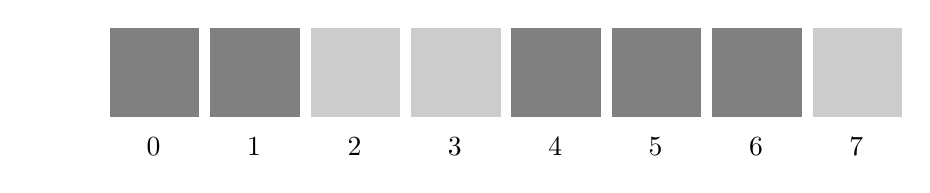
\begin{tikzpicture}[scale=.75]
\path (-1.4cm,0) -- (0,0);  % Space for robot
\foreach \n/\x/\color in
  {0/0/100, 1/1.7/100, 2/3.4/40, 3/5.1/40,
   4/6.8/100, 5/8.5/100, 6/10.2/100, 7/11.9/40} {
    \draw[fill,color=gray!\color] (\x,0) rectangle +(1.5,1.5);
    \node[xshift=.55cm] at (\x, -5mm) {\p{\n}};
}
\end{tikzpicture}
\end{center}

Para maior clareza, as portas e paredes são desenhadas como se estivessem no chão e o robô se move sobre elas, medindo a intensidade com sensores de solo.

A tarefa do robô é entrar em uma porta específica, digamos a que se encontra na posição 4. Mas como o robô pode saber onde ele está? Por odometria, o robô pode determinar sua posição atual, dada uma posição inicial conhecida. Por exemplo, se o robô estiver na extremidade esquerda da parede:
\begin{center}
% Robot trying to localize 2
\begin{tikzpicture}[scale=.75]
\path (-1.4cm,0) -- (0,0);  % Space for robot
\foreach \n/\x/\color in
  {0/0/100, 1/1.7/100, 2/3.4/40, 3/5.1/40,
   4/6.8/100, 5/8.5/100, 6/10.2/100, 7/11.9/40} {
    \draw[fill,color=gray!\color] (\x,0) rectangle +(1.5,1.5);
    \node[xshift=.55cm] at (\x, -5mm) {\p{\n}};
}
\pic[scale=.5,fill] at (-1.1cm,7.5mm) { robot };
\end{tikzpicture}
\end{center}
ele sabe que tem que se mover cinco vezes a largura de cada porta, enquanto que se o robô estiver na posição seguinte:
\begin{center}
% Robot trying to localize 3
\begin{tikzpicture}[scale=.75]
\path (-1.4cm,0) -- (0,0);  % Space for robot
\foreach \n/\x/\color in
  {0/0/100, 1/1.7/100, 2/3.4/40, 3/5.1/40,
   4/6.8/100, 5/8.5/100, 6/10.2/100, 7/11.9/40} {
    \draw[fill,color=gray!\color] (\x,0) rectangle +(1.5,1.5);
    \node[xshift=.55cm] at (\x, -5mm) {\p{\n}};
}
\pic[scale=.5,fill] at (5.5cm,7.5mm) { robot };
\end{tikzpicture}
\end{center}
a porta necessária é a próxima à direita. Devido a erros na odometria, é bem provável que com o passar do tempo o robô se perca. Nesta seção, implementamos uma versão unidimensional de um algoritmo de \emph{localização probabilístico Markov} que leva em conta a incerteza nos sensores e no movimento do robô, e retorna as localizações mais prováveis do robô.

O Apêndice~\ref{a.bayes} contém um pequeno tutorial sobre probabilidade condicional e regra Bayes, incluindo um exemplo dos detalhes dos cálculos de incerteza.

\subsection{A detecção aumenta a certeza}

Considere um robô no ambiente acima de paredes e portas que não tenha informações sobre sua localização. O robô atribui uma probabilidade para as oito posições onde ele pode estar localizado. Inicialmente, ele não tem idéia de onde está, então a cada posição será atribuída a probabilidade $b[i]=1.0/8=.125\approx .13$, onde $b$ é chamado de \emph{belief array}:\footnote{Todas as probabilidades serão arredondadas a dois dígitos decimais para exibição.}
\begin{center}
\begin{tikzpicture}
\draw (0,3) node[left] {\p{1.0}} -- node[left] {$p$} (0,0) node[left] {\p{0.0}} -- node[below,yshift=-4mm] {$b$} (8,0);
\foreach \n/\v in {0/.13, 1/.13, 2/.13, 3/.13, 4/.13, 5/.13, 6/.13, 7/.13}
  \pic { bar=\n/\v };
\foreach \n in {.5, 1.5, 4.5, 5.5, 6.5}
  \node at (\n,3) {$\bullet$};
\pic[scale=.2] at (4.4,2.5) { robot };
\end{tikzpicture}
\end{center}

Nos enredos, os pontos indicam as posições das portas e um pequeno ícone indica a posição real do robô que está virado para a direita.

Suponha agora que os sensores do robô detectam uma área cinza escura. Sua incerteza é reduzida, pois ele sabe que deve estar diante de uma das cinco portas. A matriz de crenças mostra $,2$ para cada uma das portas e $,0$ para cada uma das paredes:
\begin{center}
\begin{tikzpicture}
\draw (0,3) node[left] {\p{1.0}} -- node[left] {$p$} (0,0) node[left] {\p{0.0}} -- node[below,yshift=-4mm] {$b$} (8,0);
\foreach \n/\v in {0/.2, 1/.2, 2/.0, 3/.0, 4/.2, 5/.2, 6/.2, 7/.0}
  \pic { bar=\n/\v };
\foreach \n in {.5, 1.5, 4.5, 5.5, 6.5}
  \node at (\n,3) {$\bullet$};
\pic[scale=.2] at (4.4,2.5) { robot };
\end{tikzpicture}
\end{center}

Em seguida, o robô avança e novamente sente uma área cinza escura. Agora há apenas três possibilidades: estava na posição 0 e se moveu para 1, estava na 4 e se moveu para 5, ou estava na 5 e se moveu para 6. Se a posição inicial do robô fosse 1 ou 6, após mover-se para a direita, ele não detectaria mais uma área cinza escura, então ele não poderia ter estado lá. A probabilidade agora é de $,33$ para cada uma das três posições 1, 4, 5:
\begin{center}
\begin{tikzpicture}
\draw (0,3) node[left] {\p{1.0}} -- node[left] {$p$} (0,0) node[left] {\p{0.0}} -- node[below,yshift=-4mm] {$b$} (8,0);
\foreach \n/\v in {0/.0, 1/.33, 2/.0, 3/.0, 4/.0, 5/.33, 6/.33, 7/.0}
  \pic { bar=\n/\v };
\foreach \n in {.5, 1.5, 4.5, 5.5, 6.5}
  \node at (\n,3) {$\bullet$};
\pic[scale=.2] at (5.4,2.5) { robot };
\end{tikzpicture}
\end{center}
Após o próximo passo do robô, se ele detecta novamente uma porta, está sem dúvida na posição 6:
\begin{center}
\begin{tikzpicture}
\draw (0,3) node[left] {\p{1.0}} -- node[left] {$p$} (0,0) node[left] {\p{0.0}} -- node[below,yshift=-4mm] {$b$} (8,0);
\foreach \n/\v in {0/.0, 1/.0, 2/.0, 3/.0, 4/.0, 5/.0, 6/1.0, 7/.0}
  \pic { bar=\n/\v };
\foreach \n in {.5, 1.5, 4.5, 5.5, 6.5}
  \node at (\n,3) {$\bullet$};
\pic[scale=.2] at (6.4,2.5) { robot };
\end{tikzpicture}
\end{center}
\noindent{}Se o robô não detectou uma porta, ele está ou na posição 2 ou na posição 7:
\begin{center}
\begin{tikzpicture}
\draw (0,3) node[left] {\p{1.0}} -- node[left] {$p$} (0,0) node[left] {\p{0.0}} -- node[below,yshift=-4mm] {$b$} (8,0);
\foreach \n/\v in {0/.0, 1/.0, 2/.5, 3/.0, 4/.0, 5/.0, 6/.0, 7/.5}
  \pic { bar=\n/\v };
\foreach \n in {.5, 1.5, 4.5, 5.5, 6.5}
  \node at (\n,3) {$\bullet$};
\end{tikzpicture}
\end{center}
O robô mantém uma matriz de crenças e integra novos dados quando detecta a presença ou ausência de uma porta. Com o passar do tempo, a incerteza diminui: o robô sabe com maior certeza onde ele está realmente localizado. Neste exemplo, eventualmente o robô conhece sua posição na frente da porta $6$ com total certeza ou reduziu sua incerteza para uma das duas posições $2,7$.

\subsection{Incerteza na detecção}

Os valores retornados pelos sensores do robô refletem a intensidade da luz refletida pelas cores cinzas das portas e paredes. Se a diferença na cor de uma porta cinza escuro e uma parede cinza claro não for muito grande, o robô pode ocasionalmente detectar uma porta cinza escuro como uma parede cinza claro, ou inversamente. Isto pode ocorrer devido a mudanças na iluminação ambiente ou devido a erros nos próprios sensores. Segue-se que o robô não consegue distinguir entre os dois com total certeza.

Nós modelamos este aspecto do mundo atribuindo probabilidades à detecção. Se o robô sentir cinza escuro, especificamos que a probabilidade é de $,9$ de ter detectado corretamente uma porta e $,1$ de ter detectado erroneamente uma parede onde de fato havia uma porta. Por outro lado, se ele sentir cinza claro, a probabilidade é de $,9$ de ter detectado corretamente uma parede e $,1$ de ter detectado erroneamente uma porta onde havia uma parede.

Continuamos a exibir os cálculos em gráficos, mas você pode achar mais fácil segui-los em Tabela~\ref{tab.uncertain-sensing}. Cada linha representa a matriz de crenças do robô seguindo a ação escrita na primeira coluna.

\begin{table}
\caption[Localização com incerteza no sensoriamento]{Localização com incerteza no sensoriamento\newline{}sensor=após multiplicar pela incerteza do sensor\newline{}norm=após a normalização\newline{}direita=após mover-se para a direita uma posição}\label{tab.uncertain-sensing}
\setlength{\tabcolsep}{6pt}
\begin{tabular}{l|rrrrrrrr}
\hline\noalign{\smallskip}
posição&\multicolumn{1}{c}{$0$}&\multicolumn{1}{c}{$1$}&\multicolumn{1}{c}{$2$}&\multicolumn{1}{c}{$3$}&\multicolumn{1}{c}{$4$}&\multicolumn{1}{c}{$5$}&\multicolumn{1}{c}{$6$}&\multicolumn{1}{c}{$7$}\\
porta?&\multicolumn{1}{c}{$\bullet$}&\multicolumn{1}{c}{$\bullet$}&&&\multicolumn{1}{c}{$\bullet$}&\multicolumn{1}{c}{$\bullet$}&\multicolumn{1}{c}{$\bullet$}&\\
\hline\noalign{\smallskip}
inicial &$0.13$ & $0.13$ & $0.13$ & $0.13$ & $0.13$ & $0.13$ & $0.13$ & $0.13$\\
sensor  &$0.11$ & $0.11$ & $0.01$ & $0.01$ & $0.11$ & $0.11$ & $0.11$ & $0.01$\\
norm    &$0.19$ & $0.19$ & $0.02$ & $0.02$ & $0.19$ & $0.19$ & $0.19$ & $0.02$\\
\hline
à direita   &$0.02$ & $0.19$ & $0.19$ & $0.02$ & $0.02$ & $0.19$ & $0.19$ & $0.19$\\
sensor  &$0.02$ & $0.17$ & $0.02$ & $0.00$ & $0.02$ & $0.17$ & $0.17$ & $0.02$\\
norm    &$0.03$ & $0.29$ & $0.03$ & $0.00$ & $0.03$ & $0.29$ & $0.29$ & $0.03$\\
\hline
à direita   &$0.03$ & $0.03$ & $0.29$ & $0.03$ & $0.00$ & $0.03$ & $0.29$ & $0.29$\\
sensor  &$0.03$ & $0.03$ & $0.03$ & $0.00$ & $0.00$ & $0.03$ & $0.26$ & $0.03$\\
norm    &$0.07$ & $0.07$ & $0.07$ & $0.01$ & $0.01$ & $0.07$ & $0.63$ & $0.07$\\
\noalign{\smallskip}\hline\noalign{\smallskip}
\end{tabular}
\end{table}

Inicialmente, depois de sentir o cinza escuro em uma posição onde há uma porta, só sabemos com probabilidade $,125 por 0,9 = 0,1125$ que uma porta foi detectada corretamente; no entanto, ainda há uma probabilidade de $,125 por 0,1= 0,0125$ de ter detectado erroneamente uma parede. Depois de normalizar (Apêndice~\ref{a.normalize}), a matriz de crenças é:
\begin{center}
\begin{tikzpicture}
\draw (0,3) node[left] {\p{1.0}} -- node[left] {$p$} (0,0) node[left] {\p{0.0}} -- node[below,yshift=-4mm] {$b$} (8,0);
\foreach \n/\v in {0/.19, 1/.19, 2/.02, 3/.02, 4/.19, 5/.19, 6/.19, 7/.02}
  \pic { bar=\n/\v };
\foreach \n in {.5, 1.5, 4.5, 5.5, 6.5}
  \node at (\n,3) {$\bullet$};
\pic[scale=.2] at (4.4,2.5) { robot };
\end{tikzpicture}
\end{center}

O que acontece quando o robô move uma posição para a direita? Sua matriz de crenças também deve mover uma posição para a direita. Por exemplo, a probabilidade de $,19$ de que o robô estivesse na posição $1$ agora se torna a probabilidade de que ele esteja na posição $2$. Da mesma forma, a probabilidade de $,02$ de que o robô estivesse na posição $3$ agora se torna a probabilidade de que ele esteja na posição $4$. A probabilidade agora é de $0$ de que o robô esteja na posição $0$ e a probabilidade de $b_7$ torna-se $b_8$, de modo que os índices se tornam $1$--$8$ ao invés de $0$--$7$. Para simplificar os cálculos e os diagramas no exemplo, os índices $0$--$7$ são mantidos e o valor de $b_8$ é armazenado em $b_0$ como se o mapa fosse cíclico. A matriz de crenças depois que o robô se move para a direita é:
\begin{center}
\begin{tikzpicture}
\draw (0,3) node[left] {\p{1.0}} -- node[left] {$p$} (0,0) node[left] {\p{0.0}} -- node[below,yshift=-4mm] {$b$} (8,0);
\foreach \n/\v in {0/.02, 1/.19, 2/.19, 3/.02, 4/.02, 5/.19, 6/.19, 7/.19}
  \pic { bar=\n/\v };
\foreach \n in {.5, 1.5, 4.5, 5.5, 6.5}
  \node at (\n,3) {$\bullet$};
\pic[scale=.2] at (5.4,2.5) { robot };
\end{tikzpicture}
\end{center}

Se o robô sentir novamente cinza escuro, a probabilidade de estar nas posições 1, 5 ou 6 deve aumentar. Computando as probabilidades e normalizando dá:
\begin{center}
\begin{tikzpicture}
\draw (0,3) node[left] {\p{1.0}} -- node[left] {$p$} (0,0) node[left] {\p{0.0}} -- node[below,yshift=-4mm] {$b$} (8,0);
\foreach \n/\v in {0/.03, 1/.29, 2/.03, 3/.0, 4/.03, 5/.29, 6/.29, 7/.03}
  \pic { bar=\n/\v };
\foreach \n in {.5, 1.5, 4.5, 5.5, 6.5}
  \node at (\n,3) {$\bullet$};
\pic[scale=.2] at (5.4,2.5) { robot };
\end{tikzpicture}
\end{center}

Agora o robô se move novamente para a direita:
\begin{center}
\begin{tikzpicture}
\draw (0,3) node[left] {\p{1.0}} -- node[left] {$p$} (0,0) node[left] {\p{0.0}} -- node[below,yshift=-4mm] {$b$} (8,0);
\foreach \n/\v in {0/.03, 1/.03, 2/.29, 3/.03, 4/.0, 5/.03, 6/.29, 7/.29}
  \pic { bar=\n/\v };
\foreach \n in {.5, 1.5, 4.5, 5.5, 6.5}
  \node at (\n,3) {$\bullet$};
\pic[scale=.2] at (6.4,2.5) { robot };
\end{tikzpicture}
\end{center}
\noindent{}e sente uma terceira área cinza escura. A matriz de crenças se torna:
\begin{center}
\begin{tikzpicture}
\draw (0,3) node[left] {\p{1.0}} -- node[left] {$p$} (0,0) node[left] {\p{0.0}} -- node[below,yshift=-4mm] {$b$} (8,0);
\foreach \n/\v in {0/.07, 1/.07, 2/.07, 3/.01, 4/.0, 5/.07, 6/.63, 7/.07}
  \pic { bar=\n/\v };
\foreach \n in {.5, 1.5, 4.5, 5.5, 6.5}
  \node at (\n,3) {$\bullet$};
\pic[scale=.2] at (6.4,2.5) { robot };
\end{tikzpicture}
\end{center}
Não é surpreendente que o robô esteja quase certamente na posição 6.
\begin{framed}
\act{Localização com incerteza do sensor}{local-uncertain}
\begin{itemize}
\item Implementar a localização probabilística com incerteza no sensor.
\item Como o comportamento do algoritmo muda quando a incerteza é alterada?
\item Execute o algoritmo para diferentes posições iniciais do robô.
\end{itemize}
\end{framed}

\section{Incerteza em movimento}\label{s.uncertain-motion}

Assim como a incerteza nos sensores, os robôs estão sujeitos à incerteza em seu movimento. Podemos pedir ao robô para mover uma posição para a direita, mas ele pode mover duas posições, ou pode mover-se muito pouco e permanecer em sua posição atual. Modifiquemos o algoritmo para levar em conta esta incerteza.

Que $b$ seja a matriz de crenças. A matriz de crenças é atualizada usando a fórmula:
\begin{displaymath}
b'_i = p_i \, b_i\,,
\end{displaymath}
onde $b'_i$ é o novo valor de $b_i$ e $p_i$ é a probabilidade de detectar uma porta (no exemplo, $p_i$ é $0,9$ para $i=0,1,4,5,6$ e $p_i$ é $0,1$ para $i=2,3,7$). Se o movimento for certo, o robô move uma posição para a direita, mas com movimento incerto, o seguinte cálculo leva em conta as probabilidades de $q_j$ que o robô realmente move $j=0,1,2$ posições:
\begin{displaymath}
b'_i = p_i \,(b_{i-2}\, q_2 + b_{i-1}\, q_1 + b_{i}\, q_0)\,,
\end{displaymath}
como mostrado no diagrama a seguir:
\begin{center}
\begin{tikzpicture}[scale=1.1]
\begin{scope}[every node/.style={draw,rectangle,minimum size=1cm}]
\node (b2)  {$b_{i-2}$};
\node (b1)  [right=of b2] {$b_{i-1}$};
\node (b)   [right=of b1] {$b_{i}$};
\node (b2p) [below=of b2] {};
\node (b1p) [below=of b1] {};
\node (bp)  [below=of b]  {$b'$};
\end{scope}
\draw[->] (b2.south) -- node[below,near start] {$q_2$} (bp.north west);
\draw[->] (b1.south) -- node[above] {$q_1$} (bp.north);
\draw[->] (b.south)  -- node[above,near end,xshift=6pt] {$q_0$} (bp.north east);
\end{tikzpicture}
\end{center}
É altamente provável que o robô se mova corretamente, portanto os valores razoáveis são $q_1=0,8$ e $q_0=q_2=0,1$. Com estes valores para a incerteza do movimento e os valores anteriores para $p_i$, o cálculo da matriz de crenças após três movimentos é mostrado na Tabela~\ref{tab.uncertain-sensing-motion} e seu valor final é mostrado no diagrama a seguir:
\begin{center}
\begin{tikzpicture}
\draw (0,3) node[left] {\p{1.0}} -- node[left] {$p$} (0,0) node[left] {\p{0.0}} -- node[below,yshift=-4mm] {$b$} (8,0);
\foreach \n/\v in {0/.11, 1/.21, 2/.05, 3/.01, 4/.02, 5/.13, 6/.43, 7/.05}
  \pic { bar=\n/\v };
\foreach \n in {.5, 1.5, 4.5, 5.5, 6.5}
  \node at (\n,3) {$\bullet$};
\pic[scale=.2] at (1.4,2.5) { robot };
\node at (2,2.5) {\p{?}};
\pic[scale=.2] at (6.4,2.5) { robot };
\node at (7,2.5) {\p{?}};
\end{tikzpicture}
\end{center}
O robô está provavelmente na posição 6, mas estamos menos certos porque a probabilidade é de apenas $,43$ ao invés de $,63$. Há uma probabilidade não negligenciável de $,21$ de que o robô esteja na posição 1.

\begin{table}
\caption[Localização com incerteza na detecção e no movimento]{Localização com incerteza na detecção e no movimento\newline{}sensor=após multiplicar pela incerteza do sensor\newline{}norm=após a normalização\newline{}direita=após mover-se para a direita uma posição}\label{tab.uncertain-sensing-motion}
\setlength{\tabcolsep}{6pt}
\begin{tabular}{l|rrrrrrrr}
\hline\noalign{\smallskip}
posição&\multicolumn{1}{c}{$0$}&\multicolumn{1}{c}{$1$}&\multicolumn{1}{c}{$2$}&\multicolumn{1}{c}{$3$}&\multicolumn{1}{c}{$4$}&\multicolumn{1}{c}{$5$}&\multicolumn{1}{c}{$6$}&\multicolumn{1}{c}{$7$}\\
door?&\multicolumn{1}{c}{$\bullet$}&\multicolumn{1}{c}{$\bullet$}&&&\multicolumn{1}{c}{$\bullet$}&\multicolumn{1}{c}{$\bullet$}&\multicolumn{1}{c}{$\bullet$}&\\
\hline\noalign{\smallskip}
inicial  & $0.13$ & $0.13$ & $0.13$ & $0.13$ & $0.13$ & $0.13$ & $0.13$ & $0.13$\\
sensor & $0.11$ & $0.11$ & $0.01$ & $0.01$ & $0.11$ & $0.11$ & $0.11$ & $0.01$\\
norm     & $0.19$ & $0.19$ & $0.02$ & $0.02$ & $0.19$ & $0.19$ & $0.19$ & $0.02$\\
\hline
à direita    & $0.05$ & $0.17$ & $0.17$ & $0.04$ & $0.04$ & $0.17$ & $0.19$ & $0.17$\\
sensor & $0.05$ & $0.17$ & $0.02$ & $0.00$ & $0.03$ & $0.15$ & $0.17$ & $0.02$\\
norm     & $0.08$ & $0.27$ & $0.03$ & $0.01$ & $0.06$ & $0.25$ & $0.28$ & $0.03$\\
\hline
à direita    & $0.06$ & $0.09$ & $0.23$ & $0.05$ & $0.01$ & $0.07$ & $0.23$ & $0.25$\\
sensor & $0.05$ & $0.10$ & $0.02$ & $0.01$ & $0.01$ & $0.06$ & $0.21$ & $0.02$\\
norm     & $0.11$ & $0.21$ & $0.05$ & $0.01$ & $0.02$ & $0.13$ & $0.43$ & $0.05$\\
\noalign{\smallskip}\hline\noalign{\smallskip}
\end{tabular}
\end{table}

\begin{framed}
\act{Localização com incerteza no movimento}{local-motion}
\begin{itemize}
\item Implementar a localização probabilística com incerteza no cálculo da potência do motor.
\item Como o comportamento do algoritmo muda quando a incerteza é alterada?
\item Execute o algoritmo para diferentes posições iniciais do robô.
\end{itemize}
\end{framed}

\section{Sumário}

A odometria fornece uma estimativa da posição de um robô. Um robô pode usar técnicas de levantamento para calcular sua posição em relação a um objeto de posição conhecida. O GPS fornece excelentes dados sobre a localização, porém, pode não ser suficientemente preciso e a interferência na recepção dos satélites limita seu uso em ambientes internos. Se houver múltiplos objetos conhecidos que o robô possa detectar e se ele tiver um mapa de seu ambiente, ele pode usar a localização probabilística para estimar sua posição com alta probabilidade, embora a probabilidade seja reduzida se houver muita incerteza nos sensores ou no movimento do robô.

\section{Leitura adicional}

Os métodos probabilísticos na robótica são tratados em profundidade na  \cite{thrun}. Há uma grande quantidade de informações sobre GPS em \url{http://www.gps.gov}. Uma implementação de localização probabilística usando o robô educacional Thymio é descrita em \cite{wang2016dars}.
